%This chapter will review some important considerations when designing and implementing a virtual reality application using gesture recognition as input method.

\section{Virtual Technology}
Virtual reality can be defined as a realistic and immersive simulation of a three-dimensional 360 degree environment, 
created using interactive software and hardware, and experienced or controlled by movement of the body~\citep{VRS2016}.

One of the most common ways to experience a virtual reality is through virtual reality headsets, which are stereoscopic head-mounted displays (HMD) 
that provide separate images for each eye~\citep{POLYGON2016}. 
In addition to separate eye displays a HMD typically also contains head motion sensors such as gyroscopes, accelerometers 
and other sensors to track the user's head movements~\citep{TW2016}. 
A person using a virtual reality head-mounted display should thus perceive a virtual world with realistic depth vision and be able to "look around" 
by turning his or her head.

% The development of virtual reality head-mounted displays was in many ways fueled by the development of smart phones as many of the components are similar 
% (e.g.~gyroscopes), and
% these components also became more affordable by the prominence of smart phones. 
% This led to the prototype HMD "Oculus Rift Development Kit 1", released by Oculus VR in 2012, 
% being the first independently developed and sold virtual reality headset\citep{TW2016}. 

\begin{figure}%[h!] %[H]
	\includegraphics[width=\linewidth]{pictures/oculus_rift_dk1.jpg}
	\caption[The Oculus Rift Development Kit 1]{The Oculus Rift Development Kit 1, released by Oculus VR in 2012.}
	\label{fig:oculus}
\end{figure}


\section{The Virtual Reality Ecosystem}
As described in the previous section, a virtual reality head-mounted device (HMD) is in simple terms a device that is fastened to the user's head and, when fastened, 
covers the user's entire field of vision. 
Each eye has its own display, and both of these are positioned about 2-3 centimeters from the eyes. In addition to this, several head motion
tracking sensors are built into the headset to detect any movement~\citep{POLYGON2016}. This usually includes a gyroscope, which is responsible for measuring the orientation of the
HMD, and some times an accelerometer to measure the proper acceleration of the HMD \citep{THEVERGE2016}. In addition, or instead of this, the first consumer versions of 
virtual reality headset also usually utilizes some other sensors or cameras outside the HMD. As an example the Oculus Rift CV1 utilizes constellation sensors~\citep{VRFOCUS2015}, 
which are usually positioned on a table, while the HTC Vive utilizes two "lighthouse stations", which are usually placed in opposite corners of the room, and uses photosensors and 
structured light lasers to obtain the users position and rotation~\citep{GIZMODO2015}. 
Several virtual reality headset vendors also offer controllers that are either included or sold separately. These are usually wireless and 
utilize similar sensor technology as the head mounted devices.   

% It is worth noting that both of these virtual reality headset also is sold with their own controllers, which uses similar technology as the HMD, but as previously stated this
% thesis will investigate gesture recognition systems as the primary interaction method.  

\begin{figure}%[h!] %[H]
	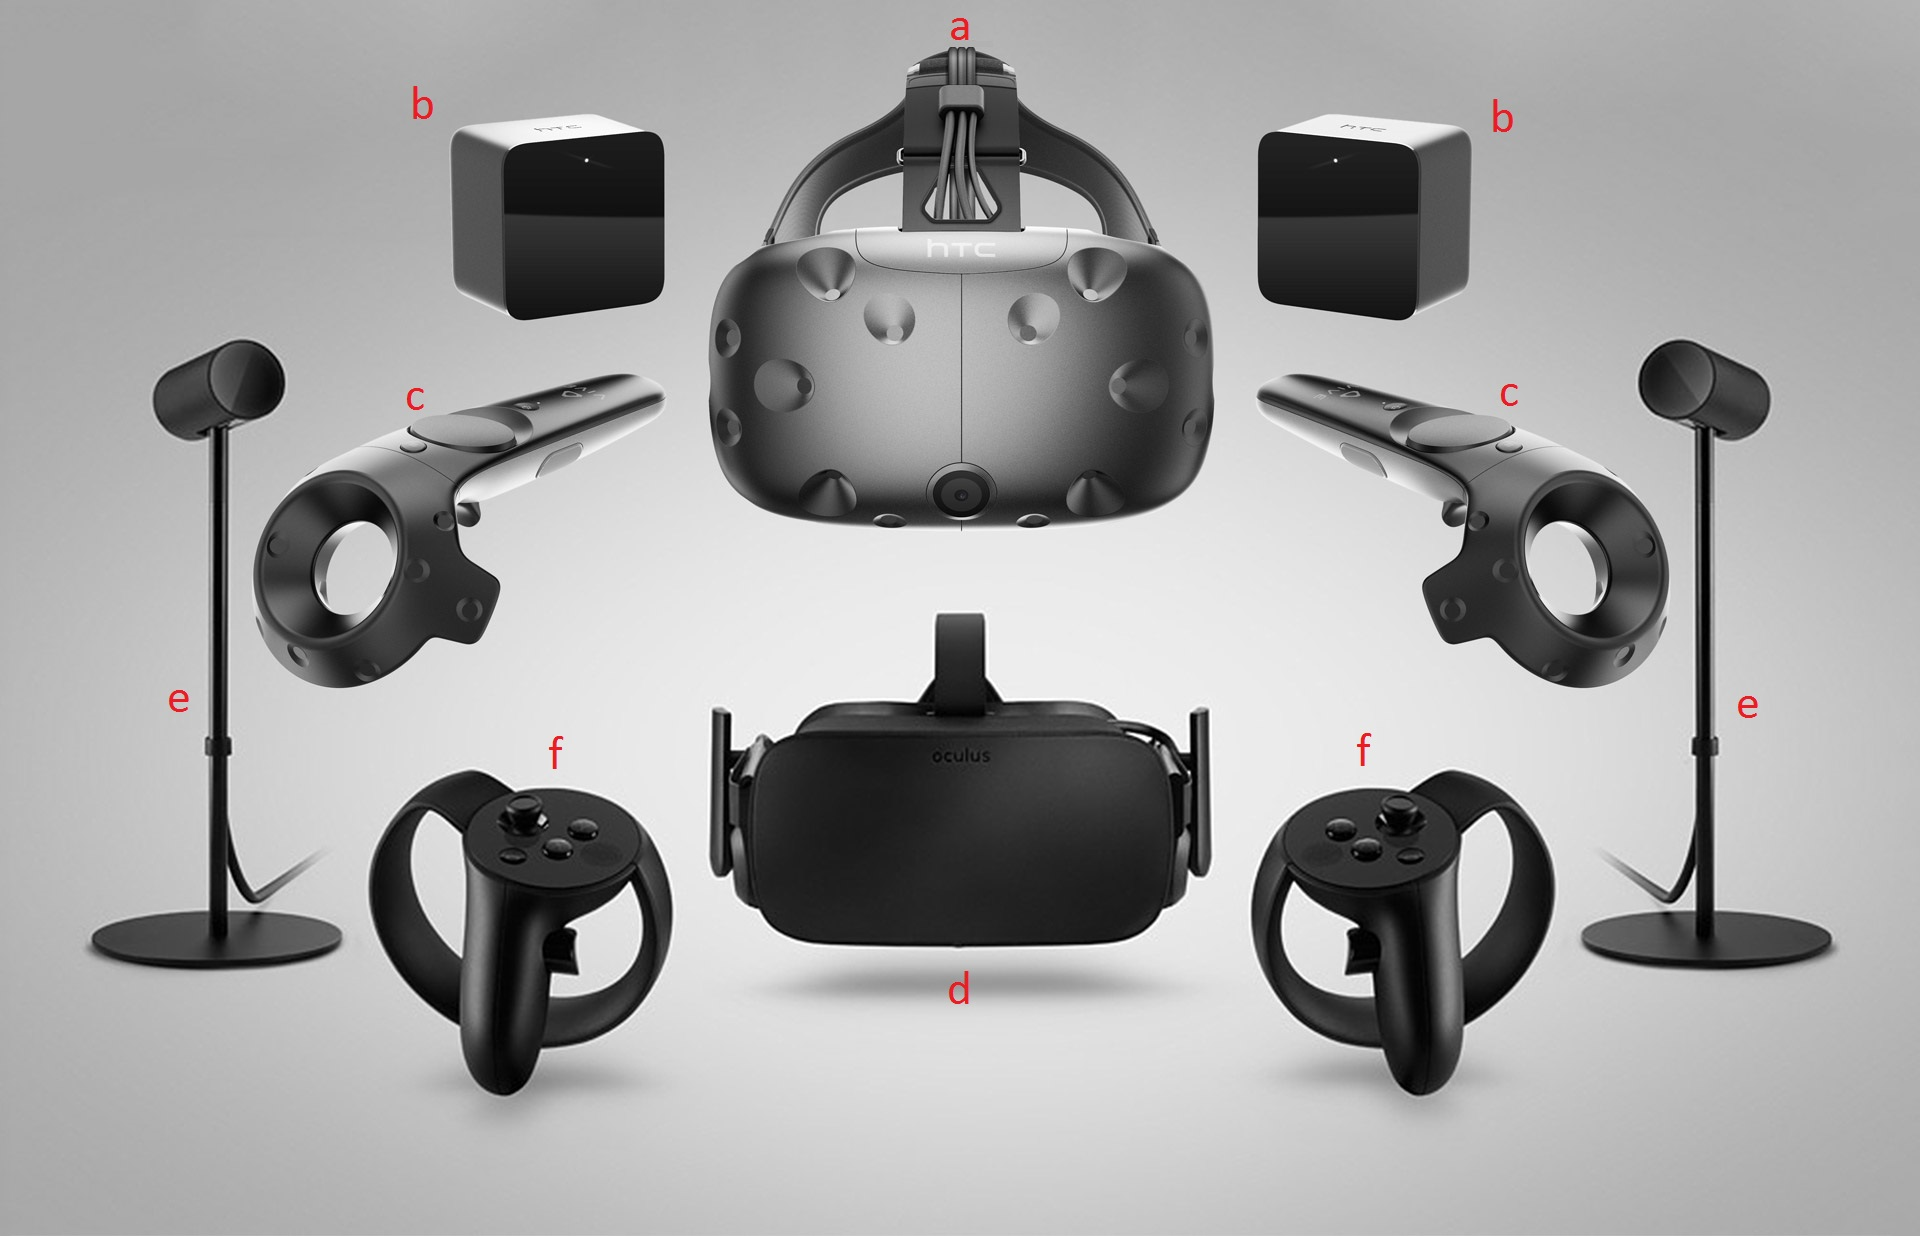
\includegraphics[width=\linewidth]{pictures/vive_and_rift_marked.jpg}
	\caption[The HTC Vive and Oculus Rift Hardware]{The HTC Vive and Oculus Rift Hardware. 
    a) The HTC Vive headset (HMD). b) The HTC Vive Lighthouse Stations. c) The HTC Vive Controllers. d) The Oculus Rift headset (HMD). e) The Oculus Rift Constellation Sensors. 
    f) The Oculus Rift Touch Controllers. Picture from \citet{ROADTOVR2016}}
	\label{fig:vive_and_rift_marked}
\end{figure} 

\section{Virtual Reality Performance Demands}
Virtual reality places some strict demands on performance and software design to avoid discomfort for the user. This is in many ways connected to how virtual reality "tricks" 
the user's brain into thinking the virtual experiences are actually real, thus giving it its "reality feel". Failing to meet these demands can quickly result in significant 
discomfort for the user, often called \textbf{\textit{virtual reality sickness}}, a kind of motion sickness~\citep{ARSTECHNICA2013}. Some of these demands are described below:

\subsection{Latency Requirements}
Virtual reality headsets have a much stricter requirements for latency, i.e the time required for an input to have a visible effect, 
than with use of regular displays~\citep{ROADTOVR2013}. If this demand isn't met the system might feel "sluggish", and user's actions and 
visual feedback might feel disjoint, which often lead to virtual reality sickness. According to one of the engineers behind the HTC Vive, the ideal
latency is between 7 and 15 milliseconds~\citep{ARSTECHNICA2013}. One important component of this latency is the \textit{refresh rates} of the displays, i.e 
how often the display hardware updates its buffers and thus "draws" a new image on the displays. As an example both the Oculus Rift CV1 and the HTC Vive
has a refresh rate of 90 Hz (i.e the display updates 90 times per second), as opposed to the 60 Hz which is more common in commodity displays.
In addition to refresh rate, the \textit{frame rate}, i.e how often the graphics processing unit (GPU) renders new frames/images, is also important. To ensure 
that the displays don't "redraw" an identical frame on a buffer update the frame rate should thus ideally be the same or higher than the refresh 
rate (e.g 90 frames per second for the Oculus Rift CV1 or HTC Vive). Refresh rate and frame rate are thus highly codependent, where performance is only as good as the weaker
of the two, and the target computer should thus have a GPU strong enough to meet a frame rate equal or above to the HMD's refresh rate. 

\subsubsection{Asynchronous Reprojection}
To reduce the perceived latency, or to compensate for a frame rate that is too low, several virtual reality HMDs make use of \textit{asynchronous reprojection}
(equivalent to what Oculus VR refer to as "asynchronous time warp")~\citep{GD2016}. This is a technique in which the virtual reality system generates intermediate frames 
in situations where the software (e.g a game) can't maintained the required frame rate (which is typically 90 fps with 90 Hz). In simple terms asynchronous reprojection 
produces "in-between frames", which is a manipulated version of an older rendered frame. This is done my morphing the frame according to the most recent head tracking data just 
before the frame is presented on the displays~\citep{GD2016}. By doing this, software that runs at e.g 45 FPS (frames per seconds) natively can be transformed into 90 FPS by 
applying asynchronous reprojection to each rendered frame. Every other frame is thus actually a manipulated version of the former frame. 

\subsection{Display Resolution and Quality}
Virtual reality headsets also have strict demands in respect to display resolution and quality. As the eyes of the user is closer
to the displays than with a regular monitor, and the displays have to "wrap around" the user's whole field of view, flaws and shortcomings in the display technology 
become more apparent. 
One such example is \textit{the screen-door effect (SDE)}, 
which is when the lines separating the display pixel or subpixels is visible in the displayed image~\citep{TC2016}. 
To illustrate this issue \citet{TC2016} had the following remark about the Oculus Rift DK1 (released in 2013 with a resolution of 640×800 per eye):

"Its low resolution screen (combined with magnification lenses that helped wrap the image around your view) made even the most beautifully rendered 3D environment look dated. 
It was like you were sitting too close to an old TV, or staring at the display through a screen door (aptly, this shortcoming quickly came to be known as “the screen door effect”)"

\begin{figure}%[h!] %[H]
	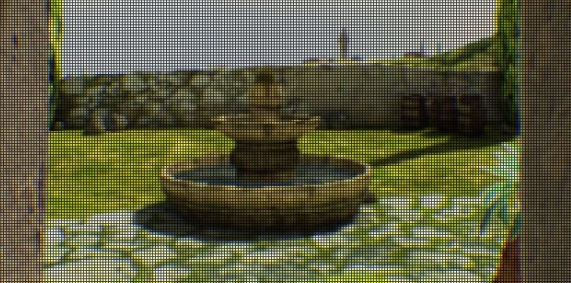
\includegraphics[width=\linewidth]{pictures/the_screen_door_effect.jpg}
	\caption[The screen-door effect]{An example of the screen-door effect.}
	\label{fig:the_screen_door_effect}
\end{figure} 

\section{Virtual Reality Sickness}
% Carsten: This is a very interesting survey of the state of knowledge in motion sickness. 
% Still, it should be motivated as well as concluded with some sentences that tell why this is an issue for your design, 
% and how the knowledge influences your design decisions. This discussion should be related to thesis goals that are already mentioned in section 1.3

As mentioned in the previous sections, virtual reality sickness, a condition similar to \textit{simulator sickness}, 
can be a consequence of the usage of virtual reality headsets, and is considered a major barrier to 
using virtual reality. Like simulator sickness, virtual reality sickness causes symptoms that are similar to those of motion sickness, and can include symptoms like 
headache, stomach awareness, nausea, vomiting, pallor, sweating, fatigue, drowsiness and disorientation~\citep{Kolasinski1995}. 
To ensure an optimal virtual reality experience when using the design review application, the design and implementation should address these issues.
The following subsection will thus review what's known about virtual reality sickness and what can be done from a design and 
implementation standpoint.


Contrary to "regular" motion sickness, where the user visually perceived to be still while in actual motion, 
virtual reality sickness turns this around: The user visually perceive to be in motion which he or she is still. 
Virtual reality sickness can thus in many ways be considered as "a reverse motion sickness". Both these condition can thus be caused by
sensory conflict, i.e that there exist a discrepancy between the information given by the senses ("the human sensors").
The susceptibility for this condition vary widely among users. Some user might experience it shortly after putting on the headset, 
while others may never experience it~\citep{Stanney2003}.
The causes for virtual reality sickness can vary and while some are less under the VR application designer's control than others, 
they should still be understood by the VR designer~\citep{Stanney2003}. 
The following two subsections will review factors that contribute to virtual reality sickness, and make a distinction by
what are mostly determined by individual differences and whats mostly determined by the application design. 

\subsection{Individual Differences in Susceptibility}
Research has identified some individual differences that correlate with the individual's susceptibility for experiencing virtual reality sickness. 
One observation is that the susceptibility for virtual reality sickness correlates heavily with motion sickness susceptibility, and 
factors that influence motion sickness susceptibility also usually influence virtual reality sickness susceptibility~\citep{Stanney2003}.
Below are some theories of the major contributing factors that are based on individual differences, and which are difficult to account for during the design of a virtual reality application.


\subsubsection{Age}
Research suggest that users between the ages of 2 and 12 are the most susceptible to virtual reality sickness~\citep{Kolasinski1995}. The susceptibility then decreases
rapidly until an age of about 21, before it start decreasing more slowly until and age of 50, where the susceptibility increases again~\citep{Brooks2010}.

\subsubsection{Gender}
Women have proven more susceptible to virtual reality sickness than men~\citep{Kennedy1985}. The most common theories to explain this difference point out the genders' differences
in hormonal composition, field of view (some research suggest that women has a wider field of view than men) and differences in depth cue recognition~\citep{Biomed2012}. 
Women are most susceptible to virtual reality sickness during ovulation~\citep{Clemes2005}.

\subsubsection{Ethnicity}
Some ethnicities seem to be more susceptible to virtual reality sickness than others, suggesting a genetic component. 
Several studies indicate that asians tends to be more susceptible to visually-induced motion sickness,
with the Chinese being more susceptible that European-Americans and African-Americans on measures to motion sickness induced by a circular vection drum, and with
Tibetans and Northeast Indians having greater susceptibility than Caucasian races~\citep{Barrett2004}.

\subsubsection{Health}
Symptoms of virtual reality sickness are more prevalent in people who are fatigued, sleep deprived, are nauseated or have an upper respiratory illness, 
ear trouble or influenza~\citep{Kolasinski1995}.

\subsubsection{Postural Stability}
Users with a postural instability has been found to be more susceptible to visually-induced motion sickness, such as virtual reality sickness, and to experience
stronger symptoms of nausea and disorientation~\citep{Kolasinski1995}. 

\subsubsection{Experience with the Application}
More exposure to virtual environments can train the brain to be less sensitive to their effects~\citep{Stanney2003}. Users tend to become less likely to experience
virtual reality sickness as they become more familiar with the virtual reality application. This adaption may occur with only a few seconds of exposure to the application~\citep{Kennedy1985}.\\


In addition to this, people with a low threshold for detecting flicker and low mental rotation ability are more susceptible to virtual reality sickness~\cite{Kolasinski1995}.

\subsection{Virtual reality design factors}
This section identifies some of the most common contributers to virtual reality sickness that can be lessened or mitigated completely by the VR application design.

\subsubsection{Acceleration}
As mentioned earlier sensory conflict during a virtual reality session might occur. This is especially noticeable during acceleration that is conveyed visually, but 
not to the vestibular organs (inner ear organs that responds to acceleration). The speed of movement does not seem to contribute to virtual reality sickness in the same scale
as the vestibular organs do not respond to constant velocity. % Needs some references

\subsubsection{Camera Control}
Some theories indicates that the ability to anticipate and control the motion the user experiences plays a significant role in staving off motion- 
and virtual reality sickness~\citep{Rolnick1991}. Unexpected movement of the camera should thus be avoided in the virtual reality application. 
If the camera control is taken away from the user it is considered good practice to cue the impending camera movement to help the user to anticipate and prepare for 
the visual motion~\citep{Lin2004}.

\subsubsection{Field of View}
The term "field of view" (FOV) can refer both to \textit{display FOV} and \textit{camera FOV}, which are similar, 
but still distinct concepts that can both have an effect on the user's proneness to virtual reality sickness. 

Display FOV refers to the area of the visual field subtended by the display. As motion perception is more sensitive in the periphery view 
a wide display FOV can contribute to VR sickness by providing the visual system with more visual input, i.e more "area" in the periphery, than a smaller display FOV. 
This can lead to more sensory conflict as more of the visual view suggest that the user is moving, which he or she might be standing or sitting still.
Reducing display FOV can reduce the changes of VR sickness \citep{Draper2001}, but can also reduce the level of immersion and awareness, and require the user to turn his or her head more
than with a higher display FOV.

Camera FOV refers the area of the virtual environment that the graphics engine draws to the display.
If the camera FOV is setup wrong, movement of the user head can lead to unnatural movement in the virtual environment (e.g a 15° rotation of the head can lead to a 
25° rotation of the camera in the virtual environment). In addition to begin highly discomforting, this can lead to a temporary impairment in the vestibulo-ocular reflex, 
which is a reflex to stabilize images on the retinas during head movement~\citep{Stanney2002}.

\subsubsection{Focus Distance}
To avoid discomfort and fatigue it is important to place content the user will be focusing on for extended amounts of time in an optimal range.
As an example Oculus VR recommends such content to be placed a distance in the range of 0.75 to 3.5 Unity units/meters away from the camera \citep{OCULUS2016}. 

\subsubsection{Latency and Lag}
As mentioned earlier in this chapter, latency and lag can have a major impact VR sickness and the usability of the virtual reality application as a whole.
Although designers and developers have no control over many aspects of a system's performance, it's important to make sure the target virtual reality application
doesn't drop frames or lag on a minimum technical specifications system~\citep{OCULUS2016}. While some dropped frames or occasional jitter can be a minor annoyance
in conventional applications or video games, it can have a much more discomforting effect on the user of a virtual reality application. 

Some research indicates that a fixed, and thus predictable, latency creates about the same degree of VR sickness whether it's as short as 48 milliseconds or as long 
as 300 milliseconds, and that big and predictable latency or lag are more comfortable for VR users than smaller, but more unpredictable, latency or lag~\citep{Draper2001}. 

\subsubsection{Mouse and Keyboard Usage}
While a user is wearing a virtual reality headset, interaction with external input devices such as a keyboard, might be inconvenient or difficult. 
Put simply, this is because the user can't see his or her hands and thus can't get the visual hand positional feedback they could get without the virtual reality HMD. 
Because of this, many virtual reality applications makes use of a gamepad controller instead. %reference needed

%\subsubsection{Distortion Correction}

%\subsubsection{Flicker}

%\subsubsection{Independent Visual Backgrounds}




